\section{Problem Formulation}
\label{sec:setup}Here we present the problem formulation for lifelong pretraining of PTLM, provide details about the data stream construction process and downstream tasks, and introduce the evaluation protocol.

% \xiang{Please work out 2 more illustrative figures:
% 1) One for illustrating the two different data streams + what we want to evaluate/analyze on the stream;
% 2) one for side by side comparing the CL baselines and KD variants}



\subsection{Lifelong Pretraining of PTLMs}
% We consider the scenario where a pretrained language model $f$ visits a sequence of $T$ (unlabeled) text corpora $D_{1..T}=\{D_1, D_2,...D_T\}$, indexed by $t$. 
We consider the scenario where one needs to deploy and/or maintain NLP models over a sequence of $T$ data domains. At each time step $t$ the model visits an unlabeled text corpus $D_t$ from a domain with a data distribution $P(D_t)$. The data distribution $P(D_t)$ evolves as the time step $t$, forming a \textit{data stream} $D_{1..T}=\{D_1, D_2,...D_T\}$. In practice, the data domain shift can refer to the topic change of the text content (from computer science research papers to biomedical papers), or temporal evolution of the text (from past to recent tweets).
The task of \textit{lifelong pretraining of PTLM} looks to continuously adapt a language model $f$ as the model visits (unlabeled) text corpus $D_t$ from the data stream $D_{1..T}$, in order to provide a good model initialization for fine-tuning on downstream tasks from the same domain. With slight abuse in notations, we also use $D_t$ to directly refer to a data domain. 

%Here, we refer to each corpus $D_t$ as a pretraining  for the language model $f$ to learn.
%Here, we also use $D_t$ to refer to the domain of the corpora for the language model $f$ to learn.
Here, we assume a language model $f$ is updated sequentially over each pretraining corpora $D_t$, without accessing the full earlier corpora $\{D_i\}_{i<t}$ in the data stream $D_{1..T}$. This aims to capture practical constraints such as privacy restriction for storing earlier data, or computation budget for training over all the text corpora in $D_{1..T}$. 
% is trained over each task, while it is prohibited to access or retrain over the full corpora from earlier tasks. The constraint is common in practice, \eg, because of privacy issues to store earlier datam and time/computation budget for retraining over all previous corpora. 
We use $f_t$ to denote the language model right \textit{after} updating on the domain $D_t$. 
In our study, $f$ is a RoBERTa-base transformer~\cite{Liu2019RoBERTaAR} and the model ($f_0$) is initialized with pretrained RoBERTa weights.

The utility of the PTLMs $\{f_t\}$ is evaluated based on their fine-tuned model performance on various downstream tasks. 
After updating on a domain $D_{i}$,
the model $f_{i}$ can be fine-tuned over downstream tasks from visited domains $D_t$ where $t \leq i$. We note the set of downstream tasks related to domain $D_t$ as $S_t = \{S_t^j\}_{j=1}^{N_t}$, assuming the number of downstream tasks is $N_t$. %$\{D_{t,j}^{\textrm{FT}}\}$ %\xiang{needs update throughout the paper}, 
% where $t$ denotes that the downstream task is related to $D_t$ and 
%The resulting fine-tuned models are further evaluated on the corresponding held-out test sets of the downstream task to help assess the model performance (more details in Sec.~\ref{ssec:evaluation_protocols}). 
%We note the performance of the fine-tuend models on the downstream task $S_t$ from a pretrained model $f_i$ as $s(f_i, S_t)$.
Note that in the fine-tuning stage, model $f_t$ has no access to any of the pretraining corpus $D_{1..T}$. 


\begin{figure}
    \centering
    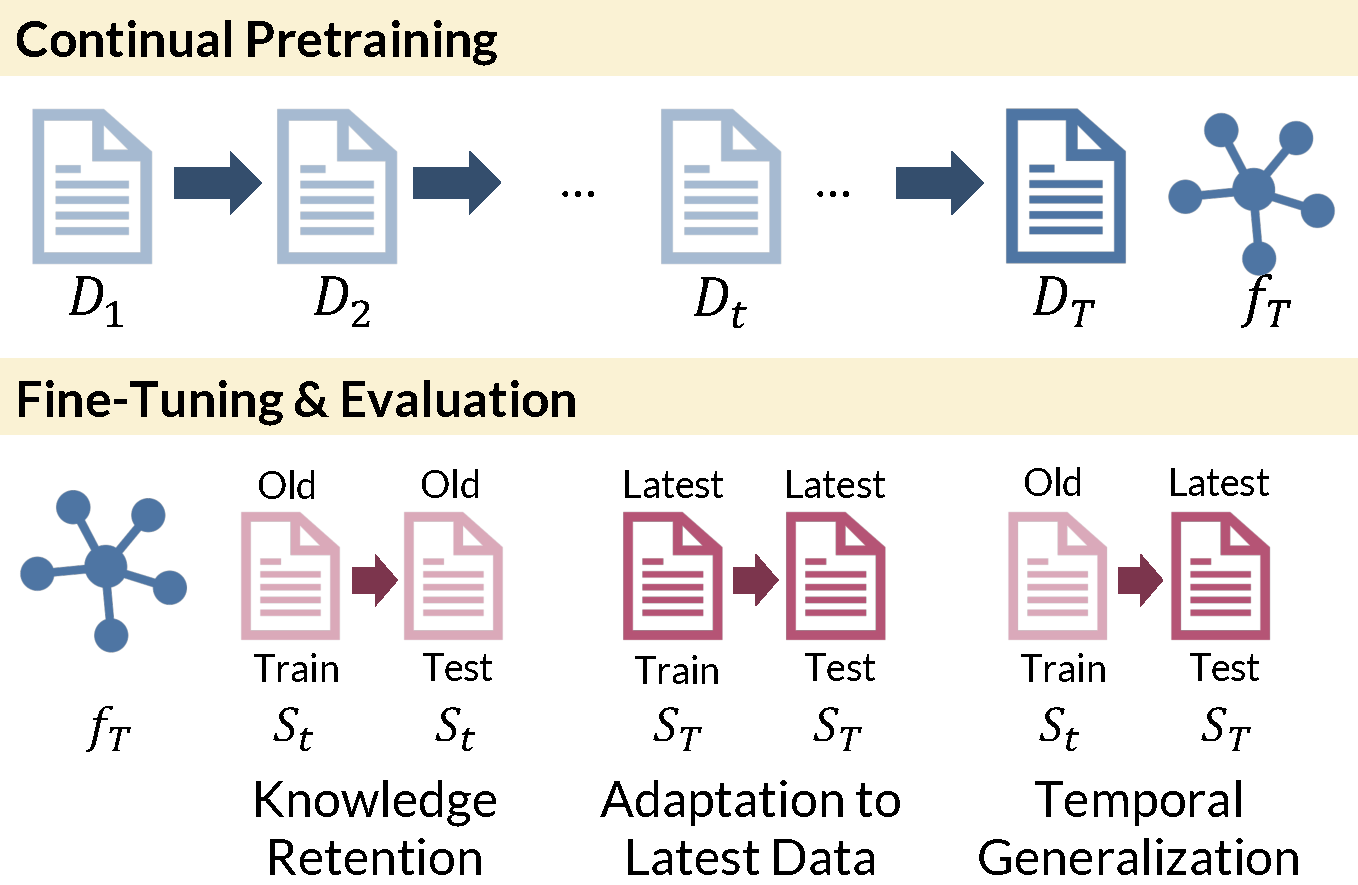
\includegraphics[width=\linewidth]{acl2022/figs/problem.pdf}
    \caption{\small \textbf{Training, evaluation setups, and metrics of lifelong language model pretraining.} The model sequentially visits each corpus, and is fine-tuned on downstream datasets related to the domains of pretraining. We evaluate knowledge retention and adaptation to new data with downstream fine-tuning performance on old and latest domains respectively. Besides, we evaluate temporal generalization where training/test examples are drawn from different time steps.
    %\xiang{need more explanation to make this figure's msgs sefl-contained. For example, I don't quite get the ``knowledge retention" and ``adaptation" part by just looking at the figure.}
   % \xiang{need to update the notations of downstream datasets.}
    }
    \label{fig:problem}
\end{figure}


\vspace{-0.1cm}
\subsection{Data Streams \& Downstream Datasets}
\label{ssec:datasets}
We construct data streams to simulate two representative scenarios of data domain shifts in practice (also see Fig.~\ref{fig:datasets}): one \textit{domain-incremental} stream to simulate the sequential changes of research paper areas; and one \textit{chronologically-ordered} stream to simulate tweets emerging over time.
% namely a domain-incremental research paper stream and a chronologically-ordered tweet stream. 
% Figure~\ref{fig:datasets} illustrates the created data streams and the evaluation focus of two data streams.


\paragraph{Domain-incremental Paper Stream.} This paper stream consists of the full text of research papers published in four research areas: biomedical, computer science, material science, and physics, filtered from the S2ORC dataset\footnote{\scriptsize{We use the 20200705v1 version of the S2ORC dataset at \url{https://github.com/allenai/s2orc}}}, which are presented sequentially to the model. For each domain, we evaluate downstream performance over two datasets. The downstream tasks span over various tasks such as relation extraction and named entity recognition, and are summarized in Table~\ref{tab:academics_downstream}. We detail these datasets in Appendix~\ref{apdx:dataset_details}. %(stat in progress)
%\xiang{any stats about \# papers in each area? Are they randomly sampled or sth else?}



\paragraph{Chronologically-ordered Tweet Stream.} 
This tweet data stream consists of tweets from the year 2014, 2016, 2018 and 2020, collected by the Archive Team\footnote{\scriptsize{\url{https://archive.org/details/twitterstream}}} and preprocessed following~\citet{nguyen2020bertweet}. These four tweet corpora are presented sequentially to the language model following the chronological order of the tweet year.
%We pre-processed the tweets by converting user names and urls to the special USER token and URL token respectively following %\xiang{why so? say a bit more}. 
For downstream tasks, we hold out 1M tweets from each year's corpus to construct multi-label hashtag prediction datasets~\cite{Gong2016HashtagRU} and single-label emoji prediction datasets~\cite{Barbieri2018SemEval2T}. On two datasets, we report label ranking average precision scores (a multi-label version of MRR) of models ~\cite{Azeemi2021COVID19TA} and Macro-F1 respectively. The detailed dataset construction process is included in Appendix~\ref{apdx:dataset_details}. 
%The label space consists of tweets containing 200 most frequent hashtags in each year. 
%We independently sample 500 tweets per label (hashtag) as training, validation and test sets, which results 10$k$ examples in each of the data splits. We also construct a 20-way single-label emoji prediction datasets following~\citet{Barbieri2018SemEval2T} with the 1M held out tweets with 5,000 tweets per emoji in each split.%, resulting in balanced datasets of the same size as the hashtag prediction datasets.
%\xiang{add a line to point to appendix for more details on the dataset construction and the full list of hashtags used in our exps.}



\subsection{Evaluation Protocol}
\label{ssec:evaluation_protocols}

% Our evaluation protocols are designed to benchmark practical usage of approaches in two axes: knowledge preservation of earlier data as well as adaptation and generalization ability to latest data.
We consider three key aspects for evaluating the utility of the language models $\{f_t\}$ that are continuously updated over the data stream $D_{1..T}$, also illustrated in Figure~\ref{fig:problem}: 
1) knowledge retention and transfer over the pretraining corpora seen earlier; 2) adaptation to the latest data domain, and 3) temporal generalization when training and evaluation data are from different time steps.

%\xiang{This subsection needs some careful revision/rewriting to clarify things and align with current analysis.}

\paragraph{Knowledge Retention.} 
%\xiang{better to first provide the high level ideas on what this aspect is about, before diving to the specific stream.}
A key utility of continual language model pretraining is to obtain a single model applicable to all domains. We focus on the evaluation of the ability with the domain-incremental paper stream, because for the tweet stream, the practical need of performance over outdated data is limited. Knowledge retention is measured with the downstream task performance from earlier or the current domains that the pretrained model has visited. More formally, for each pretrained model checkpoint in $\{f_i\}$, we fine-tune $f_i$ over downstream tasks $\{S_t\}$ where $t\leq i$ and evaluate the corresponding test set performance. It is important that the models do not suffer from catastrophic forgetting~\cite{Robins1995CatastrophicFR}, \textit{i.e.,} significantly reduced helpfulness when $f_i$ is fine-tuned for downstream tasks $S_t$ from earlier domains with $t<i$. 
%\xiang{should mention knowledge transfer too, since this is part of our analysis.}
%One major challenge in such use case is the catastrophic forgetting, \textit{i.e.,} significant performance degrade over seen domains To evaluate knowledge retention, we fine-tune a language model $f_{t}$ over downstream tasks $D_{t^\prime,j}^{\textrm{FT}}$, for each domain $t=1, ..., T$.
% from all previously seen domains. 
%We use $s(f_{t}, D_{t^\prime,j}^{\textrm{FT}})$ to denote the performance of the model fine-tuned from $f_{t}$ on $D_{t^\prime,j}^{\textrm{FT}}$. 
%\xiang{below are hard to follow; try rewrite and expand with more clear description, using notations.}
%We track the performance of the fine-tuned model on a dataset %$D_{t^\prime,j}^{\textrm{FT}}$ over the pretraining time steps $t$ ($t^\prime \leq t \leq T$) and inspect the change of the performance. 
%The forgetting is indicated by the performance degrade over the time step $t$.
%\xiang{what about knowledge transfer aspect?}% <--- this is more related to performance on latest data (below)


\begin{table}[]
\centering
\scalebox{0.65}{
\begin{tabular}{@{}llc@{}}
\toprule
Domains           & Downstream Datasets                       & Metrics  \\ \midrule
Bio-Medicine      & Chemprot~\cite{Vindahl2016ChemProt30AG}   & Micro-F1 \\
                  & RCT-Sample~\cite{Dernoncourt2017PubMed2R} & Micro-F1 \\
Comp. Science  & ACL-ARC~\cite{Jurgens2018MeasuringTE}     & Macro-F1 \\
                  & SciERC~\cite{Luan2018MultiTaskIO}         & Macro-F1 \\
Mat. Science & Synthesis~\cite{mysore2019materials}      & Macro-F1 \\
                  & MNER~\cite{olivetti2020data}              & Micro-F1 \\
Physics           & Keyphrase~\cite{augenstein2017semeval}    & Macro-F1 \\
                  & Hyponym~\cite{augenstein2017semeval}      & Macro-F1 \\ \bottomrule
\end{tabular}
}
\caption{Summary of downstream datasets relevant to each domain in the research paper stream.}
\label{tab:academics_downstream}
\vspace{-0.2cm}
\end{table}

\paragraph{Adaption to Latest Data Domain.} 
%\xiang{I think adaption is not only for tweet stream. Currently the writing mislead me about this.}
In certain scenarios, performance of downstream models over the latest data domain should be emphasized. For example, classifiers in the tweet domain are usually trained and evaluated with up-to-date data for practical deployment. Formally, we focus on the downstream task performance of models fine-tuned from the final pretrained model checkpoint $f_T$, where the downstream tasks $S_T$ are also from the latest domain. To succeed in these metrics, it is crucial for the model to transfer knowledge from earlier domains to the latest domain. 

%Over chronologically ordered data streams such as the tweet stream, it is more crucial that the model performs well over the up-to-date data instead of outdated data. 
%For this purpose, we focus on evaluating the performance on the downstream dataset $D^{\text{FT}}_{T,j}$ with the latest time step. \xiang{unclear to me.}

\paragraph{Temporal Generalization Ability.}
We consider another practical fine-tuning scenario in the tweet stream where the model is trained on outdated data and evaluated on the latest data~\cite{Rijhwani2020TemporallyInformedAO, Huang2018ExaminingTI}, referred to as the \textit{temporal generalization} ability. %The setup is prevalent to systems deployed online where collecting annotations for always up-to-date data is costly. 
Formally, we fine-tune the final pretrained model checkpoint $f_T$ over the training set of downstream tasks $S_t$ from an earlier time step ($t < T$), and evaluate on the test set of the downstream tasks $S_T$ from the latest time step $T$.
%the model is fine-tuned on outdated training examples, but evaluated on the latest test examples. 



%However, we still report performance of $f_T$ on earlier data for reference. We also evaluate whether $f_T$ improves temporal generalization ability of the model


% \textbf{Challenges}. We summarize several challenges in continual language model pretraining compared to regular continual learning. (1) first, the amount of training data is huge, which may reduce the performance of memory-replay based continual learning algorithms (2) the forgetting that happens in intermediate representations may be more crucial to the fine-tuning performance, so that continual learning algorithms that operates over model outputs may be less effective. In addition, the large output space makes it prohibitive to apply certain knowledge distillation based approaches.



\section{Methods}
\label{sec:methods}

Lifelong language model pretraining introduces novel challenges because of the large training sets and more comprehensive evaluation protocols compared to classification tasks. 
%\xiang{Here is a good place to expand the discussion on technically why this creates unique challenges as compared to CL methods applied to supervised learning.}
We establish several strong baselines, and evaluate the performance of continual learning algorithms from different categories spanning over model-expansion, memory-based, and distillation-based approaches, We illustrate the approaches in Figure~\ref{fig:method}. 

\vspace{-0.1cm}
\subsection{Simple Baselines}
\vspace{-0.1cm}
%\xiang{1) use notations to help clarify; 2) explain and motivate the purpose of including these baselines --- what insights can be brought out when comparing between them.}
We consider several simple baselines which continual learning algorithms will be compared against. \texttt{RoBERTa-base} ($f_0$) corresponds to not pretraining on any of the domain-specific corpora. By separately pretraining $f_0$ on each corpus $D_1,D_2,...D_T$, we obtain $T$ \texttt{Task-Specific} pretrained models. 
%While domain-specific models do not suffer from forgetting, they prohibit knowledge transfer between domains. 
We also pretrain $f_0$ sequentially over $D_{1..T}$, which we refer to as \texttt{sequential pretraining}. While it allows knowledge transfer between domains compared to domain-specific models, without any continual learning algorithms, sequential pretraining is prone to catastrophic forgetting~\cite{Robins1995CatastrophicFR}. Finally, we randomly shuffle corpora from all domains $D_{1..T}$ before pretraining, noted as \texttt{Multi-Task Learning (MTL)}. MTL corresponds to an offline training paradigm that models new corpora by re-training over all corpora seen before. The drawback is that it requires storing full data from earlier domains, and that it can be extremely costly to repetitively retrain over earlier data if new data keeps emerging.
%\xiang{Vanilla method is totally skipped for explanation? Which seems important because all the CL methods add on to it?}
%We also train one task specific model for each domain, noted as \texttt{Task-Specific Models}. As there can be either positive or negative knowledge transfer from other tasks, there is chance that task specific models outperform continually pretrained models.

%\xiang{multi-task learning as the reference baseline.}
%\xiang{introduce the other simple baselines we consider in the study, and also mention about the domain-specific model (``single") as a reference number (upper bound?)}

\begin{figure}
    \centering
    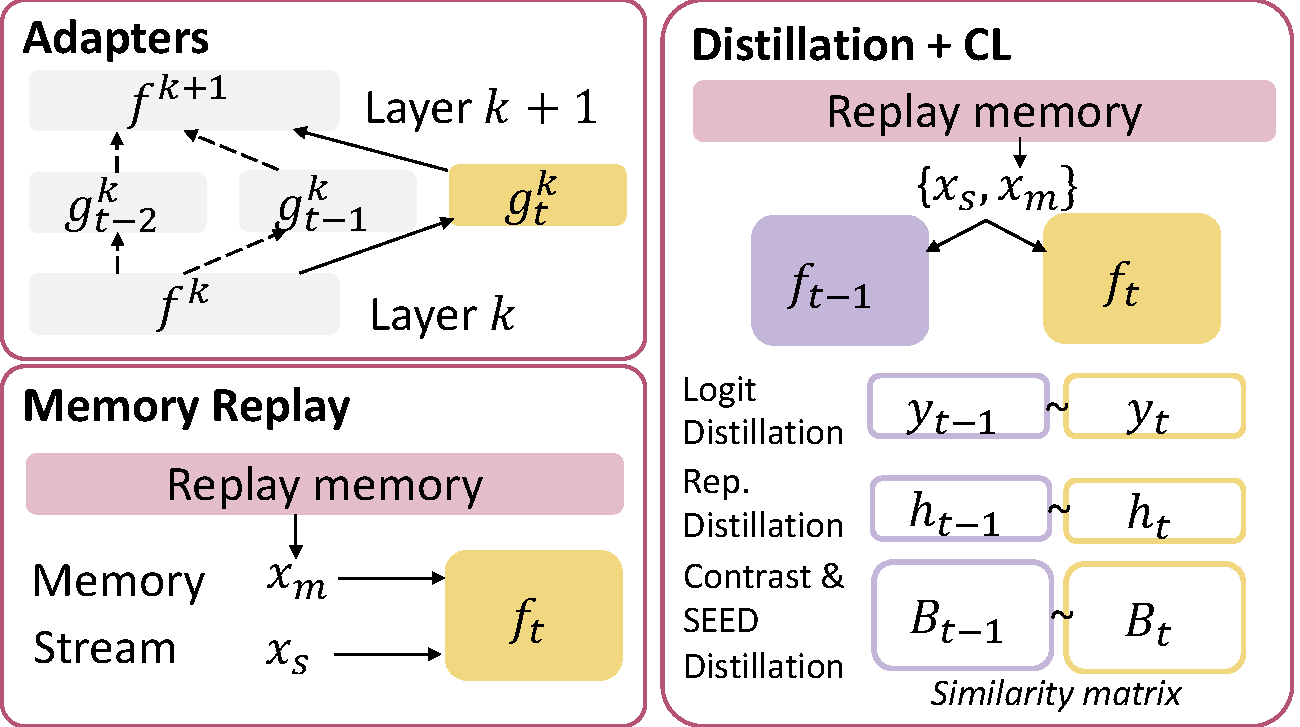
\includegraphics[width=\linewidth]{acl2022/figs/method.pdf}
    \caption{\textbf{Comparison of adapter, memory replay, and distillation-based continual learning algorithms.} 
    Details of the methods are introduced in Sec.~\ref{sec:methods}.
    %We use $g_{t}^k$ to represent adapters created for the task $t$. $\bm{x}_m$ and $\bm{x}_s$ note for the mini-batch of examples drawn from the memory and the data stream respectively.
   % \xiang{Good to include illustration on the three simple baselines.}
    }
    \label{fig:method}
\end{figure}

\vspace{-0.1cm}
\subsection{Model-expansion and Regularization-based Methods}
\vspace{-0.1cm}
%Model expansion based continual learning algorithms create new modules to model new tasks, while freezing (or discouraging change in) shared modules between tasks to prevent interference. It is non-trivial to adapt the approach to large transformer models as most of the algorithms causes significant growth of the model size. 

%\xiang{Good to have 2-3 sentences first give high level overview for this category of methods (model expansion); also can update to include the layer-specific model expansion method.}
We first introduce model-expansion based approaches, which add small trainable modules (\textit{e.g.,} multi-layer perceptron) to the model per new domain while keeping other parts of the model frozen.
The \texttt{Adapter} approach is a representative approach that learns a set of ``adapter'' layers $g_t = \{g_t^k\}_{k=1}^K$ for each domain $D_t$ and each of the $K$ transformer layers~\cite{houlsby2019parameter}. %The adapter layer is inserted between the transformer layers to modify the outputs of transformer layers $h^\prime_{k}$ as $h_{k} =  g_t^k(h^\prime_{k})$. % We implement the adapters as multi-layer perceptrons while keeping the base transformer model frozen during pretraining. 
%During fine-tuning of the language model, we apply Adapter Fusion~\cite{Pfeiffer2021AdapterFusionNT} to aggregate outputs from adapters learned for all domains $g_{1..T}$.
% allowing knowledge transfer from between domains. 
We also experiment with a simple \texttt{Layer Expansion} approach, which learns separate top two layers of the transformer and the prediction head for each domain. %During fine-tuning, we always unfreeze and fine-tune the entire weights of the model.
We also involve a regularization-based continual learning baseline, online EWC~\cite{Schwarz2018ProgressC}, which directly penalize change of model parameters. 

%. Suppose that the related downstream task is known to the model, the model may discard other adapters and only fine-tune the transformer and the corresponding adapter; while the model may also dynamically weight the output of different adapters in each layer, known as AdapterFusion.

\vspace{-0.1cm}
\subsection{Memory Replay Methods}
\label{ssec:mem_replay_methods}
\vspace{-0.1cm}
%\xiang{2-3 sentences to introduce general ideas of the memory-based approach, before diving to ER method.}
We also experiment with Experience Replay (ER)~\cite{chaudhry2019tiny}, which alleviates forgetting by storing a subset of earlier examples and periodically re-training (replaying) over them. We maintain a fixed-size memory $M$ ($100k$ examples by default) and populate the memory $M$ each time pretraining on a domain $D_t$ finishes with examples in the current domain. We ensure $M$ always contains a balanced sample of examples from all seen domains $D_{1..{t}}$. We replay a mini-batch of examples from the memory every 10 training steps.
%We apply experience replay (ER)~\cite{chaudhry2019tiny}, which alleviates forgetting by maintaining a fixed-size replay memory and regularly draw examples from the memory to replay.\xiang{tech details sound vague to me in the current writing. Need revision.}
%We maintain a memory of 100,000 examples, which are approximately 0.30\% and 0.15\% of training examples in the research paper stream and the tweet stream respectively. We populate the memory when the pretraining over the current task finishes, and randomly select examples from the current task to store in the memory. We ensure the memory always contains a balanced number of examples from all previously seen tasks. We sample a mini-batch from the memory to perform replay every 10 training steps.


\subsection{Distillation-based CL Methods}
While knowledge distillation (KD)~\cite{Hinton2015DistillingTK} techniques have been studied intensively for pretrained language models~\cite{Sun2019PatientKD}, applying them to continual learning has been under-explored outside image classification tasks~\cite{Li2018LearningWF, Rebuffi2017iCaRLIC, Hou2018LifelongLV}. Distillation based CL approaches store one previous model checkpoint of the model (noted as $f_{t-1}$) and regularize the differences between $f_{t-1}$ and the current model $f_t$.
We adapt several existing knowledge distillation techniques to PTLMs and utilize them for continual learning. We note, while individual distillation techniques are not original, their adaptation to CL algorithms can be novel.
%\xiang{below part needs adjustment as it sounds too strong and also not quite supported by exp results.}
%Not only do we expect to improve performance with these algorithms, we also hope to analyze which part of the ``dark knowledge'' in pretrained models are most important for knowledge preservation and adaptation.  %The distillation can be performed over the output logits, intermediate model representations, or leverage other information such as representational similarity between training examples. However, the issues of data-mismatch may arise as the knowledge of previous models are extracted with new data, given that examples from previous tasks are no longer available. However, algorithms show improved performance despite the mismatch issue. Other approaches may further store a small porition of previous examples to address the mismatch issue.
% \paragraph{Overall Workflow.} 

%We build distillation approaches on top of memory replay approaches. 
%Usually, knowledge distillation from a model $f_{t-1}$ requires the full training corpora where $f_{t-1}$ is pretrained on (\textit{i.e,} $D_{t-1}$). However, as CL assumes no access to the full corpora $D_{t-1}$ from earlier time steps, we maintain a memory $M$ (similar to ER) to store a subset of past examples for distillation. 
We perform distillation with examples from the current domain $D_{t}$ and a replay memory $M$ (similar to ER). 
Despite the potential gap between $D_{t}$ and the training data of $f_{t-1}$, the approach allows utilizing more data for distillation. Formally,  
each time the model receives a mini-batch of stream examples $\bm{x}_s$ or a draws mini-batch of memory examples $\bm{x}_m$ from $M$ (both noted as $\bm{x}$), we collect certain outputs of the model (\textit{e.g.}, output logits or intermediate representations) with $f_{t-1}$ and $f_t$. 
%\xiang{I got lost on what data we're operating on for doing the KD. Why do we need memory samples?}
We compute a distillation loss $\ell_{\textrm{KD}}(\bm{x}, f_{t-1}, f_t)$ that penalizes the differences between the model outputs, and jointly optimize it with the masked language modeling loss $\ell_{\textrm{MLM}}$. The final objective is written as $\ell = \ell_{\textrm{MLM}} + \alpha\ell_{\textrm{KD}}$, where $\alpha$ is a hyperparameter to weight the distillation loss. %We introduce several distillation approaches applied below.

%\xiang{can we formalize the general method a bit more with notations here? And the late part will provide more concrete tech details by referencing the notations here.}

\paragraph{Logit Distillation.} In logit distillation~\cite{Hinton2015DistillingTK}, we collect the output logits of $f_t$ and $f_{t-1}$, noted as $\bm{y}_t$ and $\bm{y}_{t-1}$ respectively. The distillation loss is computed as 
$D_{\textrm{KL}}(\bm{y}_t, \bm{y}_{t-1})$, where $D_{\textrm{KL}}$ is the Kullback–Leibler divergence function.
%the KL divergence between $\bm{y}_t$ and $\bm{y}_{t-1}$.

\paragraph{Representation Distillation.} 
We also consider minimizing the representational deviation of sentences between previous and current models~\cite{Sun2019PatientKD, Jiao2020TinyBERTDB}. We extract the representation of each word of two models, noted as $\bm{h}_{t-1}^{1:N}$ and $\bm{h}_{t}^{1:N}$, before the masked language modeling prediction head, where $N$ is the length of the sentence. Then, we compute MSE loss $\vert\vert \bm{h}_{t-1}^{1:N} -  \bm{h}_{t}^{1:N} \vert\vert_2^2$ as the distillation loss.


\begin{table*}[]
\centering
\scalebox{0.60}{
\begin{tabular}{@{}lcccccccccccc@{}}
\toprule
Task          & \multicolumn{3}{c}{$D_1$ - Biomedical} & \multicolumn{3}{c}{$D_2$ - Computer Science} & \multicolumn{3}{c}{$D_3$ - Materials Science} & \multicolumn{3}{c}{$D_4$ - Physics} \\
\cmidrule(r){1-1} \cmidrule(lr){2-4} \cmidrule(lr){5-7} \cmidrule(lr){8-10} \cmidrule(l){11-13} 
Dataset       & Chemprot           & RCT-Sample    &  MLM      & ACL-ARC               & SciERC        & MLM        & MNER                   & Synthesis    & MLM         & Keyphrase         & Hyponym     & MLM     \\ \midrule
Roberta-base  & 82.03$_{\pm 0.7}$          & 78.07$_{\pm 0.7}$    & 1.993      & 64.32$_{\pm 2.8}$             & 79.07$_{\pm 1.6}$     & 2.153        & 83.15$_{\pm 0.3}$              & 91.25$_{\pm 0.6}$        & 2.117     & 66.21$_{\pm 1.0}$         & 67.59$_{\pm 4.5}$    &   2.278  \\
Sequential Pretraining         & 82.09$_{\pm 0.5}$          & 79.60$_{\pm 0.5}$      & 1.654    & 72.73$_{\pm 2.9}$             & 81.43$_{\pm 0.8}$    & 1.807         & \textbf{83.99$_{\pm 0.3}$}              & 92.10$_{\pm 1.0}$    & 1.590          & \textbf{67.57$_{\pm 1.0}$}         & \textbf{74.68$_{\pm 4.4}$}    & \textbf{1.381}    \\
\midrule
ER            & 82.73$_{\pm 0.3}$          & 79.98$_{\pm 0.3}$  & 1.737        & 72.50$_{\pm 1.0}$             & 81.64$_{\pm 1.1}$   & 1.857           &  \textbf{83.99$_{\pm 0.4}$}              & 92.65$_{\pm 0.4}$     & 1.621        & 66.11$_{\pm 1.1}$         & 72.82$_{\pm 4.3}$   & 1.391      \\
Online EWC          & 81.83$_{\pm 0.2}$          & 78.84$_{\pm 0.5}$  & 1.655        & 71.81$_{\pm 2.6}$             & 80.79$_{\pm 0.5}$   & 1.803           &  83.43$_{\pm 0.4}$              & 91.89$_{\pm 0.5}$     & 1.571        & 66.70$_{\pm 0.6}$         & 72.98$_{\pm 6.0}$   & 1.388      \\
Adapter       & 83.30$_{\pm 0.4}$          & 80.41$_{\pm 0.4}$  & 1.417        & 69.32$_{\pm 3.5}$             & 80.22$_{\pm 1.5}$      & \textbf{1.633}       &          83.91$_{\pm 0.3}$         &    91.69$_{\pm 0.6}$    & 1.522           & 66.23$_{\pm 1.4}$         & 69.65$_{\pm 4.5}$   & 1.554     \\
Layer Expansion & 83.74$_{\pm 0.3}$ & 81.10$_{\pm 0.5}$ & \textbf{1.210} & 65.17$_{\pm 2.9}$ & 79.35$_{\pm 0.8}$  &  1.756 & 82.48$_{\pm 0.4}$ & 92.33$_{\pm 1.0}$ & 1.389 &  65.70$_{\pm 1.1}$ &  73.34$_{\pm 3.7}$ & 1.534 \\
Logit-KD      & 83.39$_{\pm 0.4}$          & \textbf{81.21$_{\pm 0.1}$}  & 1.392       & \textbf{73.70$_{\pm 3.4}$}             & 81.92$_{\pm 0.8}$      & 1.699       & 83.96$_{\pm 0.3}$              & 92.20$_{\pm 1.0}$      & \textbf{1.425}       & 64.75$_{\pm 1.1}$         & 71.29$_{\pm 3.6}$   & 1.460      \\
Rep-KD        & 82.34$_{\pm 0.3}$          & 79.59$_{\pm 0.5}$ & 1.684        & 71.17$_{\pm 2.5}$             & 78.78$_{\pm 1.1}$      & 1.810       & 84.13$_{\pm 0.3}$              & 92.02$_{\pm 0.8}$   & 1.585           &      65.96$_{\pm 1.6}$      & 73.93$_{\pm 5.5}$       &      1.389     \\
Contrast-KD   & 82.29$_{\pm 0.5}$          & 79.92$_{\pm 0.4}$  & 1.722        & 71.15$_{\pm 1.1}$             & 80.49$_{\pm 1.6}$    & 1.856         & 83.26$_{\pm 0.4}$              & 92.62$_{\pm 0.7}$   & 1.612          & 65.95$_{\pm 1.7}$         & 72.26$_{\pm 3.1}$   & 1.428     \\
SEED-KD & 82.78$_{\pm 0.3}$ & 80.38$_{\pm 0.4}$ & 1.720 & 69.98$_{\pm 2.4}$  & 81.61$_{\pm 0.7}$ & 1.829 & 82.99$_{\pm 0.4}$ & 92.35$_{\pm 0.7}$ & 1.609 & 65.35$_{\pm 1.0}$ & 74.79$_{\pm 4.1}$ & 1.401 \\ 
SEED-Logit-KD &  \textbf{83.72$_{\pm 0.4}$} & 81.05$_{\pm 0.2}$  & 1.391        & 69.90$_{\pm 4.5}$             & \textbf{83.03$_{\pm 0.6}$}   & 1.703           & 83.28$_{\pm 0.5}$              & \textbf{92.87$_{\pm 1.0}$}     & 1.428        & 65.96$_{\pm 1.5}$         & 71.92$_{\pm 5.5}$    & 1.460    \\ \midrule
Task-Specific LM        & 83.74$_{\pm 0.3}$          & 81.10$_{\pm 0.5}$    & 1.210      & 72.20$_{\pm 2.6}$             & 81.24$_{\pm 1.7}$   & 1.629          & 84.02$_{\pm 0.2}$              & 91.56$_{\pm 0.4}$        &  1.418     & 65.95$_{\pm 1.1}$         & 69.43$_{\pm 4.5}$  & 1.426      \\
MTL           & 82.91$_{\pm 1.6}$          & 80.67$_{\pm 0.4}$   & 1.289        & 69.46$_{\pm 1.8}$             & 81.12$_{\pm 0.8}$  & 1.616        & 83.92$_{\pm 0.3}$              & 92.66$_{\pm 0.6}$     &  1.355        & 65.37$_{\pm 1.6}$         & 73.31$_{\pm 5.2}$  & 1.418 \\  \bottomrule
\end{tabular}
}
\caption{\small \textbf{Results on the Research Paper stream.} We report log perplexity of MLM and the performance of downstream models fine-tuned from the final checkpoint of the pretrained model ($t=4$). Performance of the best performing CL algorithm is marked bold.
%\xiang{1) bold the 2nd best too if there's no stat signifcant difference; 2) mention p-value btw top-1 and top-2 method; 3) use up/down arrows to indicate which way the metrics are better.}
}
\label{tab:academics}
\vspace{-0.2cm}
\end{table*}
% \begin{table*}[]
% \centering
% \scalebox{0.60}{
% \begin{tabular}{@{}lcccccccccccc@{}}
% \toprule
% Task            & \multicolumn{6}{c}{Task 1 - Biomedical}                               & \multicolumn{4}{c}{Task 2 - Computer Science}                 & \multicolumn{2}{c}{Task 3 - Materials Science} \\
% \cmidrule(r){1-1} \cmidrule(lr){2-7} \cmidrule(lr){8-11} \cmidrule(l){12-13} Dataset         & \multicolumn{3}{c}{Chemprot}      & \multicolumn{3}{c}{RCT-Sample}    & \multicolumn{2}{c}{ACL-ARC}   & \multicolumn{2}{c}{SciERC}    & MNER                   & Synthesis             \\ \cmidrule(r){1-1} \cmidrule(lr){2-4} \cmidrule(lr){5-7} \cmidrule(lr){8-9} \cmidrule(lr){10-11} \cmidrule(lr){12-12} \cmidrule(l){13-13}
%  Evaluated After & Task 1    & Task 2    & Task 3    & Task 1    & Task 2    & Task 3    & Task 2        & Task 3        & Task 2         & Task 3       & Task 3                 & Task 3                \\ \midrule
% Roberta-base    & {82.03$_{\pm0.7}$}    & {82.03$_{\pm0.7}$} & {82.03$_{\pm0.7}$} & {78.07$_{\pm0.7}$}  & {78.07$_{\pm0.7}$}  & {78.07$_{\pm0.7}$}     & {64.32$_{\pm2.8}$} & {64.32$_{\pm2.8}$} & {79.07$_{\pm1.6}$} & {79.07$_{\pm1.6}$} & 83.15$_{\pm0.3}$              & 91.25$_{\pm0.6}$             \\
% Naive           & \textbf{83.74}$_{\pm0.3}$ & 82.60$_{\pm0.3}$ & 83.37$_{\pm0.5}$ & \textbf{81.10}$_{\pm0.5}$ & 80.49$_{\pm0.3}$ & 80.63$_{\pm0.3}$ & \textbf{73.71}$_{\pm2.8}$     & 69.93$_{\pm2.2}$     & 82.14$_{\pm1.1}$      & 80.70$_{\pm0.8}$    & 83.34$_{\pm0.3}$              & 92.72$_{\pm1.0}$             \\
% ER              & \textbf{83.74}$_{\pm0.3}$ & 82.96$_{\pm0.3}$ & 83.50$_{\pm0.6}$ & \textbf{81.10}$_{\pm0.5}$ & 80.79$_{\pm0.4}$ & 81.04$_{\pm0.1}$ & 69.92$_{\pm1.6}$     & 69.09$_{\pm2.1}$     & 82.01$_{\pm0.9}$      & 80.59$_{\pm0.2}$    & 83.79$_{\pm0.4}$              & \textbf{93.20}$_{\pm0.2}$             \\
% %Adapter-Single  & {83.68$_{\pm0.3}$} &  {83.68$_{\pm0.3}$} &  {83.68$_{\pm0.3}$} & {80.72$_{\pm0.7}$} & {80.72$_{\pm0.7}$} & {80.72$_{\pm0.7}$}    & {68.02$_{\pm2.6}$} & {68.02$_{\pm2.6}$} & {81.60$_{\pm0.8}$} & {81.60$_{\pm0.8}$} &    {84.15$_{\pm0.3}$}                  &      {91.11$_{\pm0.2}$}                 \\ 
% Adapter  & 83.68$_{\pm0.3}$ & 83.03$_{\pm0.4}$ &  83.19$_{\pm0.6}$      & 80.72$_{\pm0.7}$ & 80.63$_{\pm0.7}$ &     80.64$_{\pm0.5}$      & 73.28$_{\pm3.9}$     &         67.60$_{\pm 5.7}$      & 79.79$_{\pm1.5}$      &    80.10$_{\pm 1.0}$          &    \textbf{83.94}$_{\pm 0.4}$                    &          90.82$_{\pm 3.3}$         \\
% Rep-KD          & \textbf{83.74}$_{\pm0.3}$ &        82.24$_{\pm 1.0}$        &    82.90$_{\pm 0.3}$      & \textbf{81.10}$_{\pm0.5}$ &   80.60$_{\pm 0.2}$   &     80.51$_{\pm0.3}$      &       70.68$_{\pm 2.1}$        &     69.93$_{\pm 2.6}$      &      80.45$_{\pm 1.4}$       &       79.58$_{\pm 0.7}$       &     83.89$_{\pm 0.4}$                   &      92.16$_{\pm 0.6}$          \\
% Contrast-KD     & 83.38$_{\pm0.3}$ &    82.39$_{\pm 0.4}$       &    83.06$_{\pm 0.2}$     & 81.00$_{\pm0.3}$ &      80.39$_{\pm0.4}$      &   80.53$_{\pm 0.4}$     &       75.34$_{\pm 2.1}$       &    69.94$_{\pm 1.9}$       &         80.85$_{\pm 1.1}$       &      \textbf{82.45}$_{\pm 0.9}$        &          83.21$_{\pm 0.3}$          &            92.05$_{\pm 0.4}$           \\ 
% Logit-KD        & \textbf{83.74}$_{\pm0.3}$ & \textbf{83.04}$_{\pm0.2}$ & \textbf{84.12}$_{\pm0.4}$ & \textbf{81.10}$_{\pm0.5}$ & \textbf{81.26}$_{\pm0.4}$ & \textbf{81.19}$_{\pm0.2}$ & 70.72$_{\pm2.7}$     & \textbf{71.38}$_{\pm1.8}$     & \textbf{82.74}$_{\pm0.5}$      & 80.93$_{\pm0.8}$    & 83.54$_{\pm0.2}$              & 92.73$_{\pm1.0}$             \\
% \cmidrule(r){1-1} \cmidrule(lr){2-4} \cmidrule(lr){5-7} \cmidrule(lr){8-9} \cmidrule(lr){10-11} \cmidrule(lr){12-12} \cmidrule(l){13-13}

% Task-Specific LM          & \multicolumn{3}{c}{83.74$_{\pm0.3}$}     & \multicolumn{3}{c}{81.10$_{\pm0.5}$}     & \multicolumn{2}{c}{72.20$_{\pm2.6}$} & \multicolumn{2}{c}{81.24$_{\pm1.7}$} &        84.02$_{\pm 0.2}$                &         91.56$_{\pm 0.4}$              \\
% \bottomrule
% \end{tabular}
% }
% \caption{Performance of downstream models fine-tuned from continually pre-trained language models on the multi-domain research paper stream. Performance of the best performing CL algorithm is marked bold.}
% \label{tab:academics}
% \end{table*}



\paragraph{Contrastive Distillation.}
% \xiang{1) can try to compress down this part by 30\% if possible. Seems a bit too heavy on space; 2) It's important to speak out up front what differences in terms of intuitions this method bring as compared to the other KD methods.}
In addition to output logits and hidden representations, we further look into \textit{representational similarity within a batch of examples} as additional knowledge to distill. The approach is adapted from~\cite{Cha2021Co2LCC}, which is originally studied for supervised image classification tasks. %The approach consists of two components: learning a representation space with unsupervised contrastive learning, and regularize the change of representation similarity between examples.
We briefly introduce the adapted algorithm and leave the details in Appendix~\ref{apdx:cl}.
During continual pretraining, in addition to the language model pretraining objective, we add an unsupervised contrastive learning objective, namely the SimCSE~\cite{Gao2021SimCSESC} objective
%, so that the similarity in the sentence representation better 
to encourage sentence representations to reflect semantic similarities between sentences. Then, we compute the intra-batch representational similarity matrices of sentence representations (\textit{i.e.} between each pair of examples in the mini-batch) with $f_{t-1}$ and $f_t$, noted as $\mathbf{B}^{t-1}$ and $\mathbf{B}^{t}$, and minimize the cross entropy loss $\ell_{\text{distill}} = - \frac{1}{N} \sum_{i=1}^{N} \sum_{j=1}^{N} \mathbf{B}_{ij}^{t-1}\log \mathbf{B}_{ij}^{t}$
%\begin{equation}
%    \label{eq:contrastive_distill}

%\end{equation}.

% We use the $l^2$-normalized representation of the start-of-sequence token at the final layer as the sentence representation, noted as $\bm{h}$. Then, we distill the intra-batch representational similarity from the previous model $f_{t-1}$ to the current model $f_t$. Given a mini-batch of $N$ examples $\bm{x}$, we compute the representational dot-product similarity matrix between normalized sentence representations $\bm{h}$ between each pair of examples with $f_{t-1}$ and $f_t$, noted as $\mathbf{B}^{t-1}$ and $\mathbf{B}^{t}$, where each element $\mathbf{B}_{ij}$ is, 
% \begin{equation}
%     \label{eq:normalize}
%     \mathbf{B}_{ij} = \frac{\exp(\bm{h}_i \cdot \bm{h}_j / \tau)}{\sum_{k=1..N}\exp(\bm{h}_i \cdot \bm{h}_k / \tau)}
% \end{equation}
% where $\tau$ is a temperature hyperparameter. We specify a temperature $\tau_t$ for the teacher model $f_{t-1}$ and a temperature $\tau_s$ for the student model $f_t$ separately. We compute the cross-entropy between $\mathbf{B}^{t-1}$ and $\mathbf{B}^{t}$ as the distillation loss,
% \begin{equation}
%     \label{eq:contrastive_distill}
%     \ell_{\text{distill}} = - \frac{1}{N} \sum_{i=1}^{N} \sum_{j=1}^{N} \mathbf{B}_{ij}^{t-1}\log \mathbf{B}_{ij}^{t}
% \end{equation}

\paragraph{Self-Supervised Distillation (SEED).} SEED distillation proposed by~\cite{Fang2021SEEDSD} has a similar spirit as the contrastive distillation. The only difference is that it distills representational similarity \textit{between the batch and a large set of other examples}. We leave the details of the algorithm in Appendix~\ref{apdx:cl}. %As the number of target examples $K$ can be much larger than the batch size, it allows distillation of richer information by regularizing similarities. During pretraining, the method maintains a fixed-size queue $Q$ to cache examples from the current domain $D_t$. Given a mini-batch of training examples $\bm{x}$, it computes cosine similarity between each pair of examples within the batch $\bm{x}$ and $Q$ with $f_{t-1}$ and $f_{t}$, resulting in two similarity matrices $\mathbf{P^{t-1}}$, $\mathbf{P^t} \in \mathbb{R}^{|B|\times |Q|}$. Similar to the contrastive distillation, the distillation loss is the cross-entropy between two similarity matrices $\mathbf{P}^{t-1}$ and $\mathbf{P}^{t}$ computed in the same way as Eq.~\ref{eq:contrastive_distill}. 
We further combine SEED Distillation%, which empirically performs best in retaining knowledge on the research paper stream compared to Contrastive Distillation and Representation Distillation
with logit distillation and refer to the approach as SEED-Logit Distillation.

% In SimCSE, the positive pair is defined as the representations of the same sentence using different dropout masks, while the negative pairs in the mini-batch consist of representations of different sentences within the mini-batch. Let $z$, $z^\prime$ be two random dropout masks. The SimCSE loss is written as,
% \begin{equation}
% \label{eq:simcse}
% \ell_{\textrm{con}} = - \alpha \log \frac{e^{\textrm{cos-sim}(\bm{h}_i^{z_i}, \bm{h}_i^{z_j})/\tau}}{\sum_{j=1}^N e^{\textrm{cos-sim}(\bm{h}_i^{z_i}, \bm{h}_j^{z_j^\prime})/\tau}}
% \end{equation}
% where $N$ is the number of examples in the mini-batch, $\bm{h}_i^{z_i}$ is the sentence representation of an instance $i$ after dropout, $\tau$ is a temperature hyperparameter, $\alpha$ is weighting hyperparameter to the masked language modeling loss. Following the original work, we use the representation of the start-of-sequence (\texttt{<s>}) token as the sentence representation. 


% \textbf{Regularizing Similarity between Examples}. We collect the subset of task-$t$ examples selected to be stored in the memory right after learning task $t$. We group these examples with a group size equals to the batch size, noted as $B$, and note each group as $X_j = \{\hat{x}_{ij}\}_{i=1}^B$. We compute a pair-wise similarity matrix $M_j^{|B| \times |B|}$ for each group of examples and store them in the replay. In future training, we randomly select a group of examples to replay, while simutaneuously discourage the change of similarity matrix $M^\prime_j$ computed with the current model. More specifically, when a group $X_j$ is chosen for replay, in addition to the MLM loss, we added a KL divergence loss $\ell_{reg}=KL(M_j, M^\prime_j)$ that measures distance betweene similarity matrices. The KL divergences uses the same temperature hyperparemter $\tau$ and Eq.~\ref{eq:simcse}.


% \section{Datasets}
% \subsection{Pretraining datasets}
% \label{ssec:pt_datasets}
% In the current stage of the project, we included three data streams study, namely the academic papers dataset, mixed-domain dataset, and the twitter data stream.

% \textbf{Research papers dataset} consists of open-access research papers from biomedical, computer science, physics and material science domains. The dataset is a subset of S2ORC dataset\footnote{\url{https://github.com/allenai/s2orc}}~\citep{Lo2020S2ORCTS} released under CC-BY-NC 2.0. In our main experiments, we assume the model sequentially visits biomedical, computer science, physics and material science domains

% \textbf{Mixed-domain dataset} consists of four domains: biomedical research papers, computer science research papers, new articles, and amazon reviews, where has been applied in~\citep{Gururangan2020DontSP}. Here, biomedical and computer science research papers are from the same source as above. Realnews dataset~\citep{Zellers2019DefendingAN} is obtained via a google form at~\url{https://github.com/rowanz/grover/tree/master/realnews} and the license is pasted in Table~\ref{tab:license_realnews}. The amazon reviews dataset is a public dataset accessible at~\url{https://nijianmo.github.io/amazon/index.html}.



% \textbf{Twitter Data Stream}. 
% Following~\cite{Nguyen2020BERTweetAP}, we pretrain the model over the twitter data stream grabbed by the Archive Team\footnote{\url{https://archive.org/details/twitterstream}}, ranging from 01/2012 to 04/2020. 

% \subsection{Downstream Fine-Tuning Datasets}
% We fine-tine the models over a number of downstream fine-tuning tasks after pretraining. We summarize downstream datasets applied in Table~\ref{tab:downstream}. In addition, in the future we may construct our own manually labeled dataset over the pretraining datasets (introduced in Sec.~\ref{ssec:pt_datasets})
